% Created 2022-02-22 Tue 18:33
% Intended LaTeX compiler: pdflatex
\documentclass[11pt]{article}
\usepackage[utf8]{inputenc}
\usepackage[T1]{fontenc}
\usepackage{graphicx}
\usepackage{longtable}
\usepackage{wrapfig}
\usepackage{rotating}
\usepackage[normalem]{ulem}
\usepackage{amsmath}
\usepackage{amssymb}
\usepackage{capt-of}
\usepackage{hyperref}
\author{Darpan Ganatra}
\date{}
\title{Systems Biology General notes}
\hypersetup{
 pdfauthor={Darpan Ganatra},
 pdftitle={Systems Biology General notes},
 pdfkeywords={},
 pdfsubject={},
 pdfcreator={Emacs 27.1 (Org mode 9.6)}, 
 pdflang={English}}
\begin{document}

\maketitle

\section{Background}
\label{sec:orgb20e9b8}
\subsection{Protein Kinase}
\label{sec:org9bb2383}
A kinase (enzyme which catalyzes the transfer of phosephate groups from high-energy molecules to substrates) which modifies other proteins by adding phosephates to them (process of phosphorolation)
\begin{figure}[htbp]
\centering
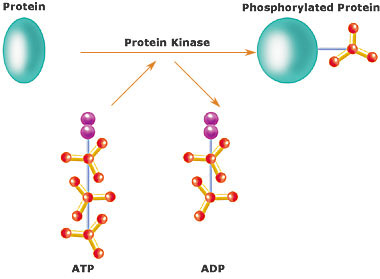
\includegraphics[width=.9\linewidth]{./Ch4_kinases.jpg}
\caption{Protein kinase (Source: Wikipedia)}
\end{figure}

\subsection{Mitogen-activated protein kinase (MAPK)}
\label{sec:orgee93c72}
\begin{itemize}
\item MAPKs are \uline{protein kinases} which are specific to serine and threonine amino acids. They're helpful in directing cellular responses to stimuli including but not limited to:
\begin{itemize}
\item Migotens
\item Osmotic Stress
\item Heat shock
\item Proinflammatory cytokines
\end{itemize}
\item These proteins are only present in eukaryotes
\item Belong to the CMGC kinase groups
\item 3 MAPK familes have been characterized:
\begin{enumerate}
\item Classical MAPK (ERK)
\item C-JunN-terminal kinase / stress-activated protein kinase (JNK/SAPK)
\item p38 kinase
\end{enumerate}
\item MAP kinases lie within protein kinase cascades
\item Each cascade has at least 3 enzlyes activated in series/sequence:
\begin{enumerate}
\item MAPK kinase kinase (MAPKKK) - At least 14
\item MAPK kinase (MAPKK) - At least 7
\item MAP kinase (MAPK) - At least 12
\end{enumerate}
\end{itemize}

\section{MAPK/ERK Pathway <-> MAPK-inase Pathway}
\label{sec:orgbe1d176}
\begin{itemize}
\item \href{https://youtube.com/watch?v=https://www.youtube.com/watch?v=r7GoZ9vFCY8}{MAP-Kinase (MAPK) signalling pathway and cancer mutation}
\end{itemize}
\end{document}
